% --------------------- VARIABLEN -------------------------

\newcommand{\COURSE}{Physik und Materialwissenschaften\\ Praktikum Physik \\}
\newcommand{\SEMESTER}{Elektro- und Informationstechnik II}
\newcommand{\STUDENT}{Maximilian Spahn\\ und\\Benjamin Langer}

\newcommand{\HEADDING}{Praktikum Physik}
\newcommand{\SUBHEADDING}{Versuch 5.3: Prismenspektroskopie}

% ------------------- DEFINITIONEN -----------------------

\documentclass[a4paper]{scrartcl}

\usepackage[utf8]{inputenc}
\usepackage[ngerman]{babel}
\usepackage{amsmath}
\usepackage{amssymb}
\usepackage{color}
\usepackage{tikz}
\usepackage{float}
\usetikzlibrary{arrows,decorations.markings}
\usepackage{tabularx}
\usepackage{fancybox}
\usepackage{pgfplots}
\usepackage[colorlinks=false,linkcolor=black,urlcolor=blue,bookmarks,bookmarksopen=true]{hyperref}
\usepackage{geometry}
\usepackage{fancyhdr}
\usepackage{subcaption}

\usepackage[page]{totalcount}

%Größe der Ränder setzen
\geometry{a4paper,left=2cm, right=2cm, top=3cm, bottom=2cm, headheight=8cm}

%Kopf- und Fußzeile
\pagestyle {fancy}
\fancyhf{}
\fancyhead[L]{\STUDENT}
\fancyhead[C]{\COURSE}
\fancyhead[R]{\today}

\fancyfoot[L]{\SEMESTER}
\fancyfoot[C]{}
\fancyfoot[R]{Seite \thepage /\pageref{LastPage}}

%Formatierung der Überschrift, hier nichts ändern
\def\header#1#2{
	\begin{center}
		{\Large #1}\\
		{#2}
	\end{center}
}

\numberwithin{equation}{subsection} 

\nocite{*}
\bibliographystyle{plainurl}

\setlength\parindent{0pt}

% ----------------------- DOCUMENT ---------------------------

\begin{document}

\vspace{10pt}
\header{\HEADDING}{\SUBHEADDING}
	
\tableofcontents
	
\newpage
	
\section{Einleitung}
Der Versuch zur Prismenspektroskopie soll die Brechung elektromagnetischer Wellen an einem Prisma zeigen.
Dafür werden Lichtspektren unterschiedlicher Leuchtdioden untersucht.

\newpage
\section{Theorie}
Licht ist eine elektromagnetische Welle, das weitreichende Spektrum mit den verschiedenen Wellenlängen ist in Abbildung \ref{fig:LichtSpektrum} dargestellt.
Unter Licht wird meist jedoch nur der sichtbare Bereich verstanden, welcher sich von ultraviolett mit einer Wellenlänge $\lambda_{untere\;Grenze} = 400\;nm$bis zu rot mit einer Wellenlänge von $\lambda_{obere\;Grenze} = 750\;nm$ erstreckt.
Jede Farbe, welche das menschliche Auge sehen kann, hat seine eigene Wellenlänge. (siehe Abbildung \ref{fig:sichtbaresLicht}) \cite{anl}

\begin{figure}[H]
	\includegraphics[width=12cm]{Abbildungen/Lichtspektrum}
	\centering
	\caption{Spektrum elektromagnetischer Wellen \cite{anl}}
	\centering
	\label{fig:LichtSpektrum}
\end{figure}

In Abbildung \ref{fig:sichtbaresLicht} ist noch einmal der sichtbare Bereich von Licht dargestellt.
Links von der Farbe violett gelangt man in den ultravioletten (UV) und rechts von rot in den infrarot (IR) Bereich. \cite{anl}
Jeder Wellenlänge kann auch eine Frequenz $f$ zugeordnet werden, indem man
die Lichtgeschwindigkeit $c$ durch die Wellenlänge $\lambda$ teilt:

\begin{align}
	f = \frac{c}{\lambda}
\end{align}

\begin{figure}[H]
	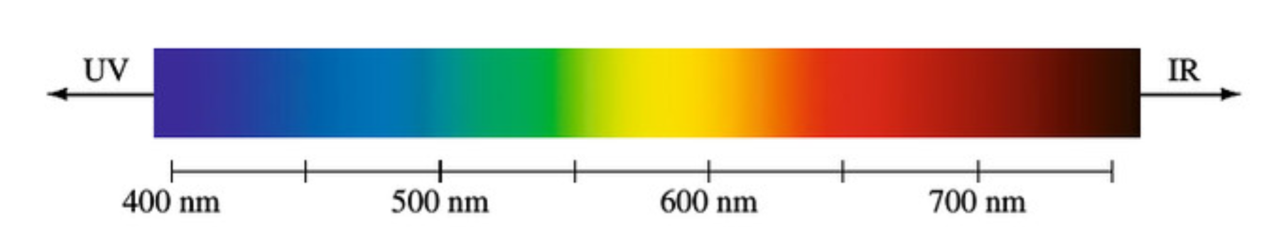
\includegraphics[width=12cm]{Abbildungen/sichtbaresLicht}
	\centering
	\caption{Bereich des sichtbaren Lichts \cite{anl}}
	\centering
	\label{fig:sichtbaresLicht}
\end{figure}

Um nun verstehen zu können, wie ein Prisma funktioniert, muss man noch wissen, dass jede Wellenlänge einen unterschiedlichen Berechungsindex hat.
Dieser Index $n$ kann über die Lichtgeschwindigkeit im Vakuum $c_0$ und über die Lichtgeschwindigkeit im Medium $c$ folgendermaßen bestimmt werden:

\begin{align}
	n = \frac{c_0}{c} \quad \cite{anl}
\end{align}
\newpage
Im Folgenden its es hilfreich sich die Abbildung \ref{fig:Brechung} genauer zu betrachten.
Wenn Licht von einem Medium in ein anderes Medium eindringt (hier von Luft mit Brechungsindex $n_1$ in Wasser mit $n_2$), bricht es an der Oberfläche nach dem Brechungsgesetz von \textbf{Snellius} (wenn die Brechungsindizes unterschiedlich sind) wie folgt:

\begin{align}
	n_1\sin(\vartheta_1) = n_2\sin(\vartheta_2)\quad \cite{hering}
\end{align}

\begin{figure}[H]
	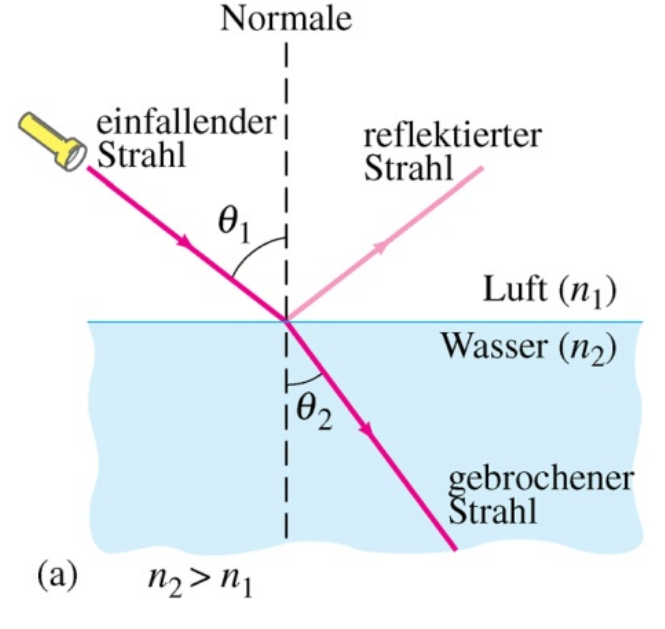
\includegraphics[width=8cm]{Abbildungen/Brechung}
	\centering
	\caption{Brechung eines Lichtstrahls \cite{anl}}
	\centering
	\label{fig:Brechung}
\end{figure}

Einen Blick auf die Abbildung \ref{fig:DispersionPrisma} zeigt, dass die Brechung bei kürzeren Wellenlängen zunimmt.
Folglich ist somit die Brechung von violettem (sichtbaren) Licht am größten.

\begin{figure}[H]
	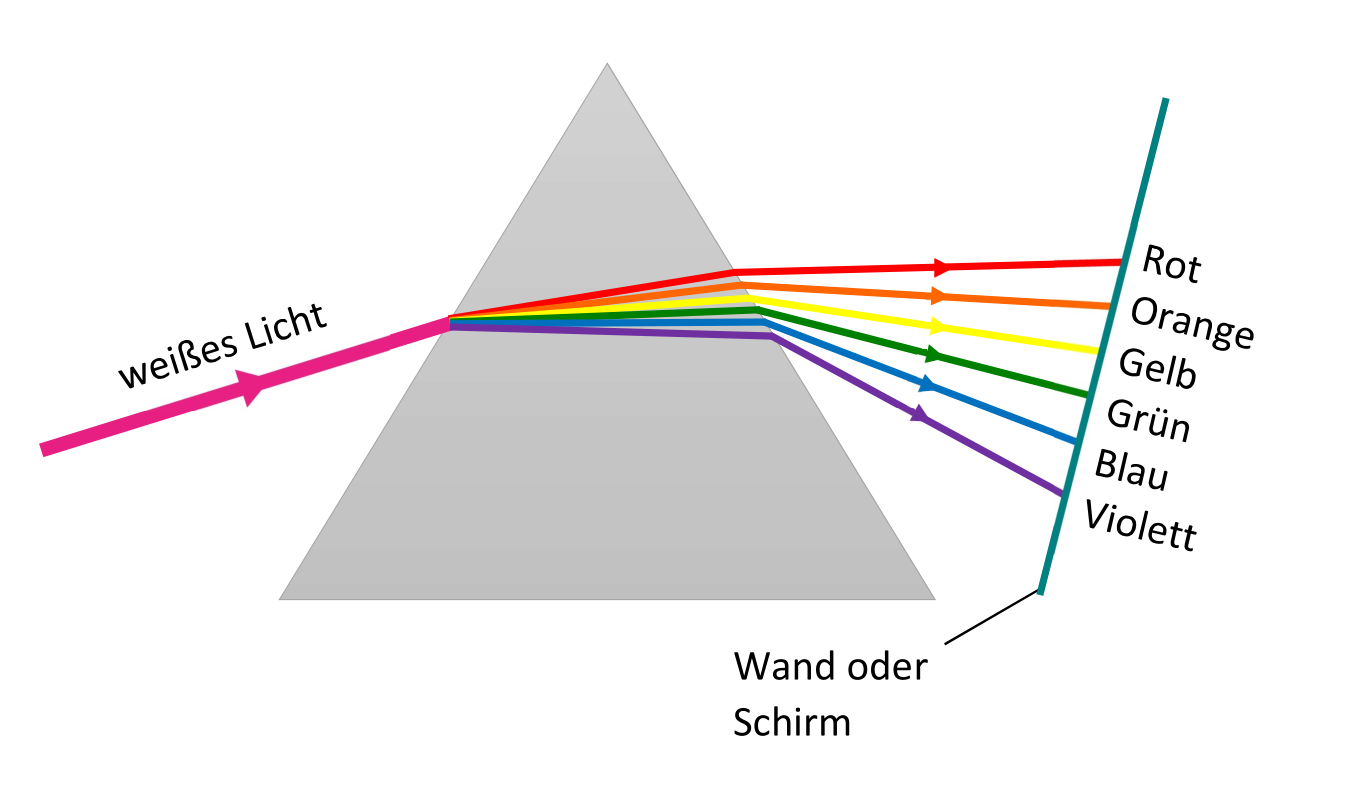
\includegraphics[width=10cm]{Abbildungen/DispersionPrisma}
	\centering
	\caption{Dispersion eines Prismas \cite{anl}}
	\centering
	\label{fig:DispersionPrisma}
\end{figure}

\newpage
\section{Häusliche Vorarbeit}
\subsection{Wie funktioniert eine LED?}
Eine Leuchtdiode (LED) besteht aus 2 Halbleiterschichten, welche in Durchlassrichtung geschaltet sind.
Durch Anlegen einer Spannung wandern Elektronen von der n-dotierten über den pn-Übergang zur p-dotierten Seite.
Dabei geht das Elektron in das energetisch günstigere Valenzband (höheres Energieniveau) über.
Ein Strom fließt durch die Diode und die aufgebaute Diffusionsspannung wird abgebaut.
Die dadurch freiwerdende Energie wird in Form von Licht (Photon) von der Diode ausgesandt.
Dabei hängt die Wellenlänge des ausgestrahlten Lichtes vom Halbleitermaterial und der Dotierung ab. \cite{leifiled}

\subsection{Warum emittiert eine Gasentladungslampe ein Linienspektrum?}
Die Gasentladung in der Lampe entsteht auf Grund von Ionisationsvorgängen.
Wenn man die an den Elektronen anliegende Spannung erhöht, werden die Elektronen immer schneller zur Anode beschleunigt.
Treffen sie auf ihrem Weg mit Neotronen zusammen, können die Elektronen aus den Atomhüllen herausschlagen (elastischer Stoß) und ionisiert werden.
Wird die anliegende Spannung an der Gasentladungslampe immer weiter erhöht, erlangen die Ladungsträger immer größere kinetische Energie, wodurch der Ionisationsvorgang einsetzt.
Man spricht auch von Stoßionisation.
Die ionisierten Elektronen hinterlassen ein Loch auf ihrer Schale.
Ein Elektron fällt auf ein energieniedrigeres Niveau herunter und sendet Licht in Form eines Photons aus.
Dies geschieht gequantelt, da es nur bestimmte Energieniveaus gibt.
Die entstehenden Emissions-Spektrallinien bilden ein Linienspektrum aus. \cite{lernhelfer}

\subsection{Unter welchem Winkel $\vartheta_1$, $\vartheta_2$ treten die beiden Wellenlängen aus dem Prisma aus?}
Ein paralleles Bündel von Lichtstrahlen, das die beiden Wellenlängen $\lambda_1 = 450\; nm$ und $\lambda_2 = 650\; nm$ enthält, tritt in ein Prisma mit dem Einfallswinkel $\gamma = 45^\circ$ ein.\\
\quad\\
Brechungsindizes:
\begin{align*}
n(\lambda_1) = 1,643 \\
n(\lambda_2) = 1,617
\end{align*}

\begin{figure}[H]
	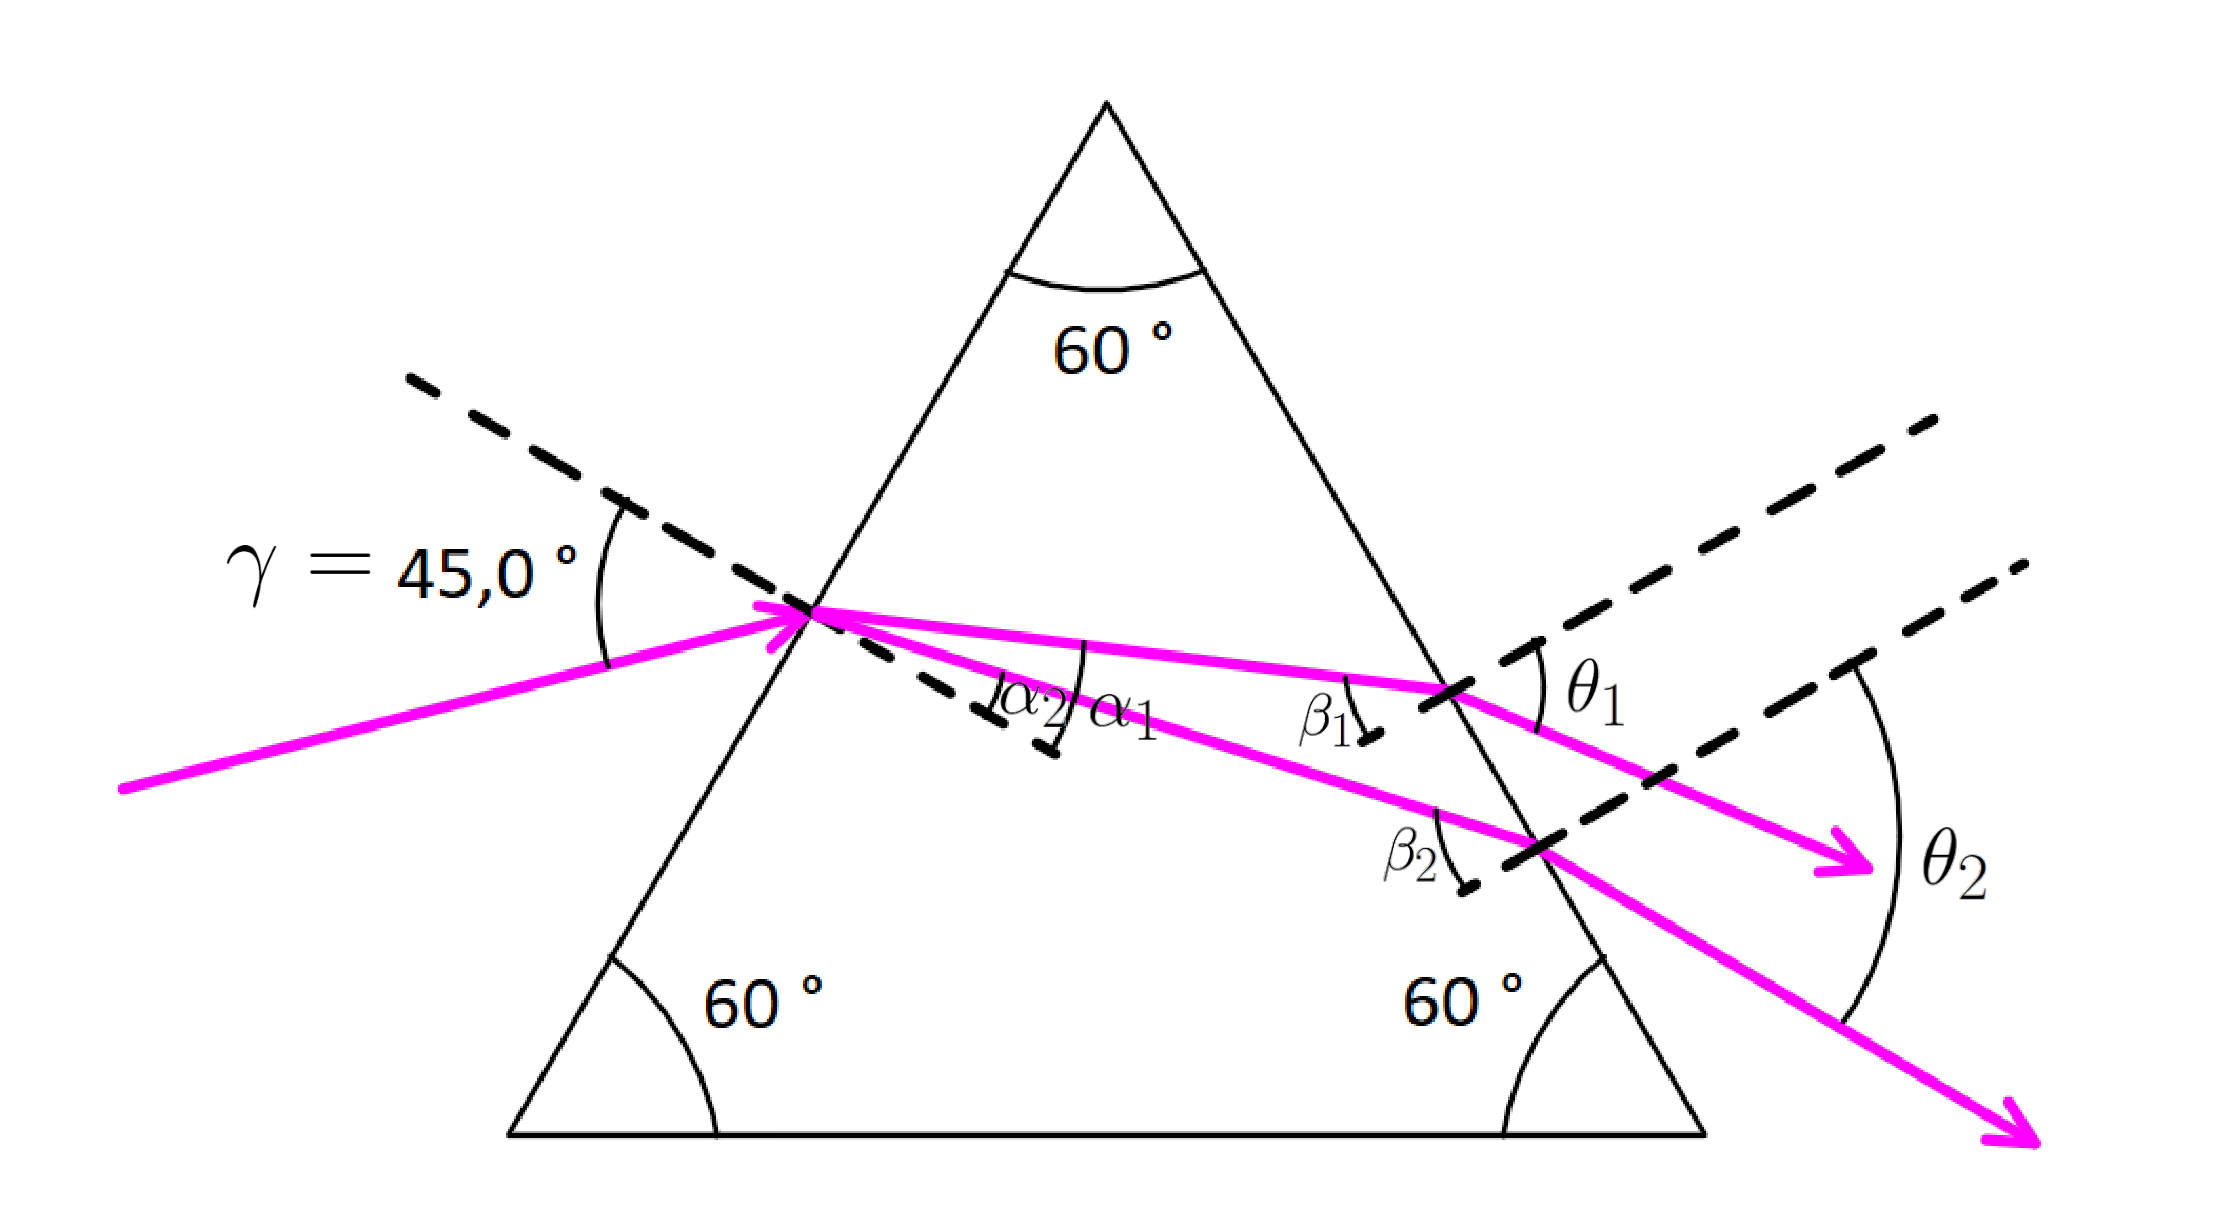
\includegraphics[width=12cm]{Abbildungen/Prisma}
	\centering
	\caption{Doppelte Lichtbrechung Prisma}
	\centering
	\label{fig:AufgabePrisma}
\end{figure}

Berechnung von $\vartheta_1$:
\begin{align*}
	n_{Luft}\sin(\gamma) &= n(\lambda_1)\sin(\alpha_1) \\
	\alpha_1 &= \arcsin\left(\frac{\sin(45^\circ)}{1,643}\right) \\
	\alpha_1 &= 25,49^\circ \\
	\quad \\
	90^\circ - 25,49^\circ &= 64,51^\circ \\
	180^\circ - 60^\circ - 64,51^\circ &= 55,49^\circ \\
	90^\circ - 55,49^\circ &= \beta_1 = 34,51^\circ \\
	\quad \\
	n(\lambda_1)\sin(\beta_1) &= n_{Luft}\sin(\vartheta_1) \\
	\vartheta_1 &= \arcsin(1,643^\circ \cdot \sin(34,51^\circ)) \\
	\vartheta_1 &= 68,57^\circ
\end{align*}

Berechnung von $\vartheta_2$:
\begin{align*}
	n_{Luft}\sin(\gamma) &= n(\lambda_2)\sin(\alpha_2) \\
	\alpha_2 &= \arcsin\left(\frac{\sin(45^\circ)}{1,617}\right) \\
	\alpha_2 &= 25,93^\circ \\
	\quad \\
	90^\circ - 25,93^\circ &= 64,07^\circ \\
	180^\circ - 60^\circ - 64,07^\circ &= 55,93^\circ \\
	90^\circ - 55,93^\circ &= \beta_2 = 34,07^\circ \\
	\quad \\
	n(\lambda_2)\sin(\beta_2) &= n_{Luft}\sin(\vartheta_2) \\
	\vartheta_2 &= \arcsin(1,617^\circ \cdot \sin(34,07^\circ)) \\
	\vartheta_2 &= 64,94^\circ
\end{align*}
\newpage
\subsection{Welches Glas ist für die Verwendung in einem Prismenspektrometer am besten geeignet?}
Das Borate flint glass ist am besten geeignet, da die Kombination aus hohem Brechungsindex und einer relativ linearen Kennlinie am höchsten ist.
(Siehe Abbildung \ref{fig:Dispersion})

\begin{figure}[H]
	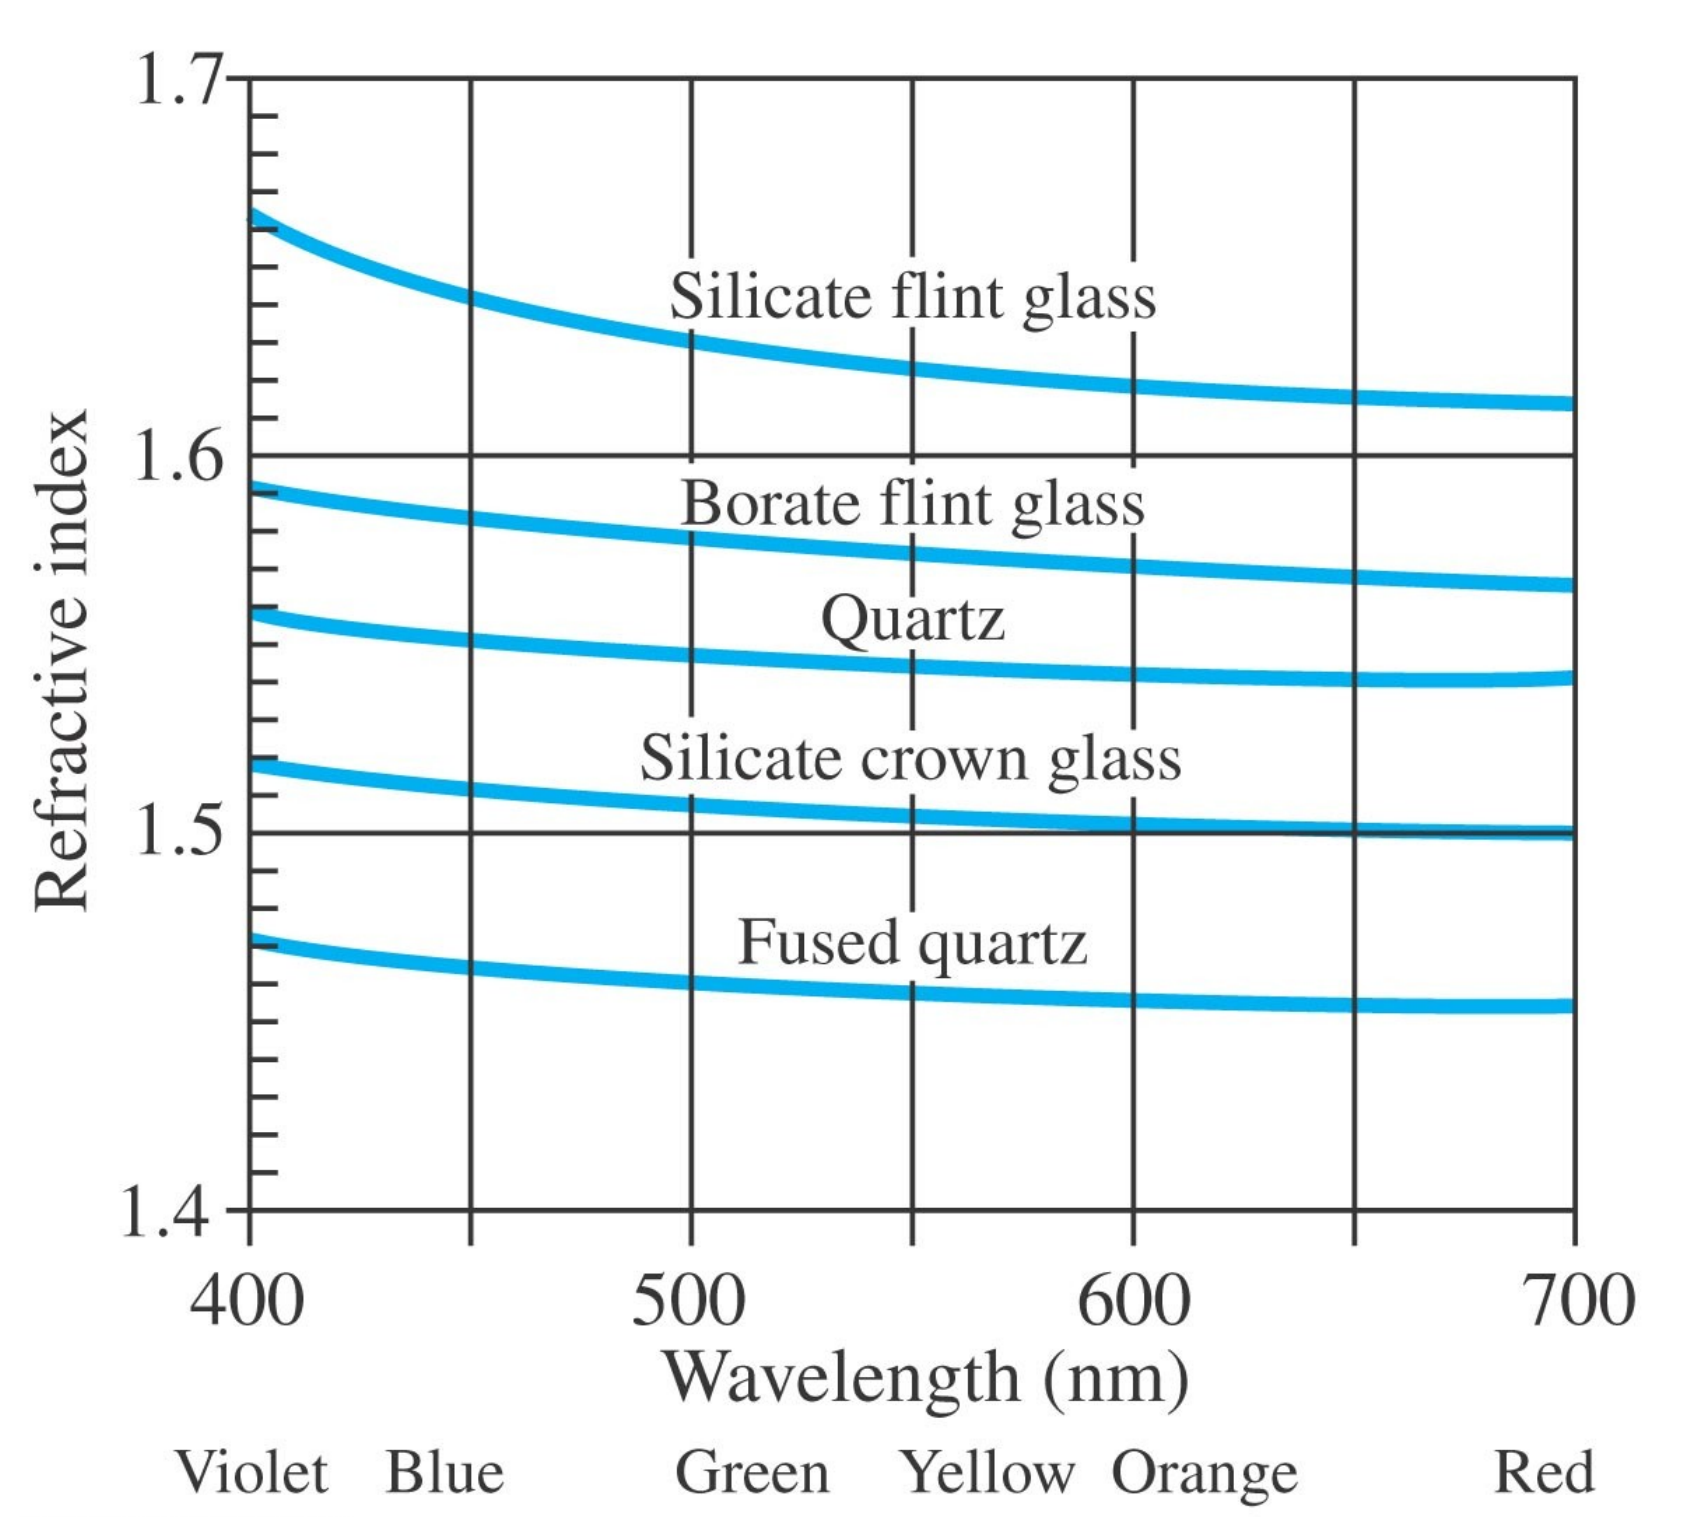
\includegraphics[width=10cm]{Abbildungen/Dispersion}
	\centering
	\caption{Dispersion \cite{anl}}
	\centering
	\label{fig:Dispersion}
\end{figure}

\subsection{Ermittlung des Winkels anhand vom Nonius}
Der Winkel von 47$^\circ$ 38' lässt sich anhand der Abbildung \ref{fig:Nonius} wiefolgt ablesen:
Der Nullzeiger vom Nonius (unterer Schieber) zeigt zwischen die 47,5$^\circ$ und die 48$^\circ$.
Dadurch hat man schonmal die vorder Zahl vor dem Gradzeichen (47$^\circ$).
Um die Winkelminuten zu ermitteln schaut man nun, wo ein unterer Strich genau mit einem oberen übereinstimmt.
Das ist bei der rot eingekreisten Ellipse der Fall und man liest 8' (Winkelminuten) ab.
Da wir davor schon über die 0,5$^\circ$ waren addieren wir 30' dazu.
Somit erhalten wir 47$^\circ$ 38'.

\begin{figure}[H]
	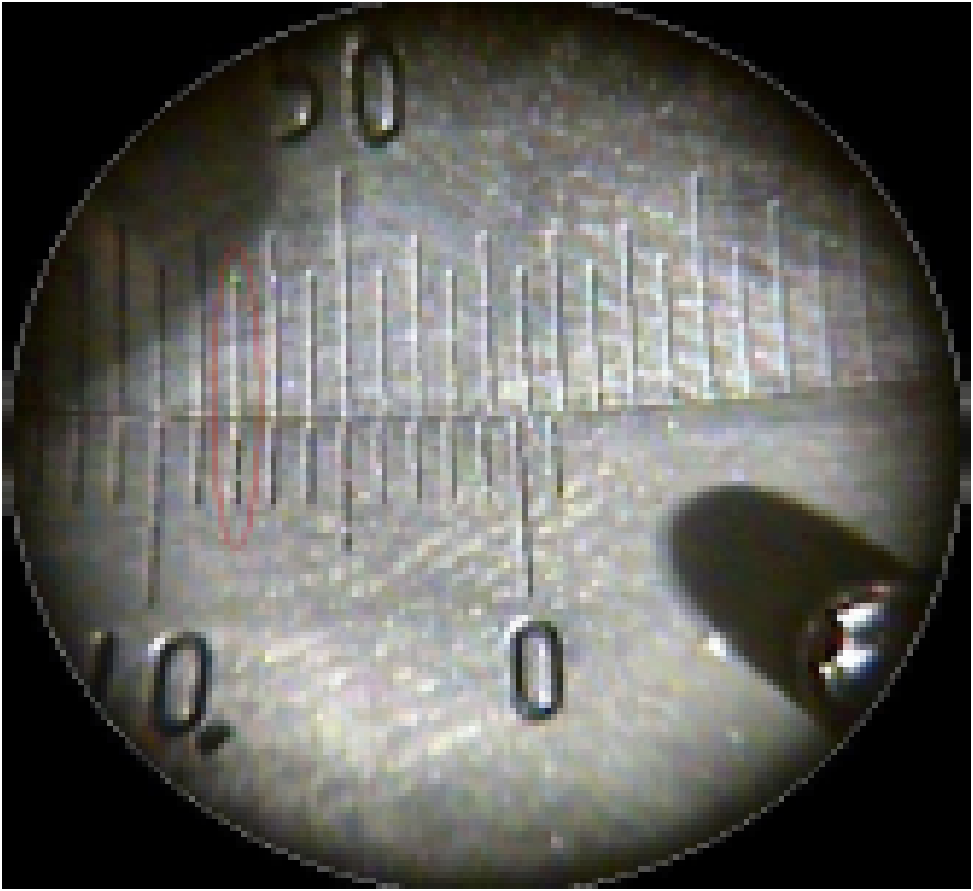
\includegraphics[width=6cm]{Abbildungen/Nonius}
	\centering
	\caption{Nonius \cite{anl}}
	\centering
	\label{fig:Nonius}
\end{figure}

\newpage
\section{Aufbau und Durchführung}
\subsection{Aufbau}
In Abbildung \ref{fig:Aufbau} ist der Aufbau zum Versuch Prismenspektroskopie dargestellt.
Durch das Spaltrohr fällt Licht auf das Prisma, welches das Licht in die Emissions-Spektrallinien zerlegt.
Sichtbar werden die einzelnen Spektrallinien (Farben) über das Fernrohr.
Anhand der Teilkreisschreibe kann dann der dazugehörige Winkel der Wellenlänge abgelesen werden.

\begin{figure}[H]
	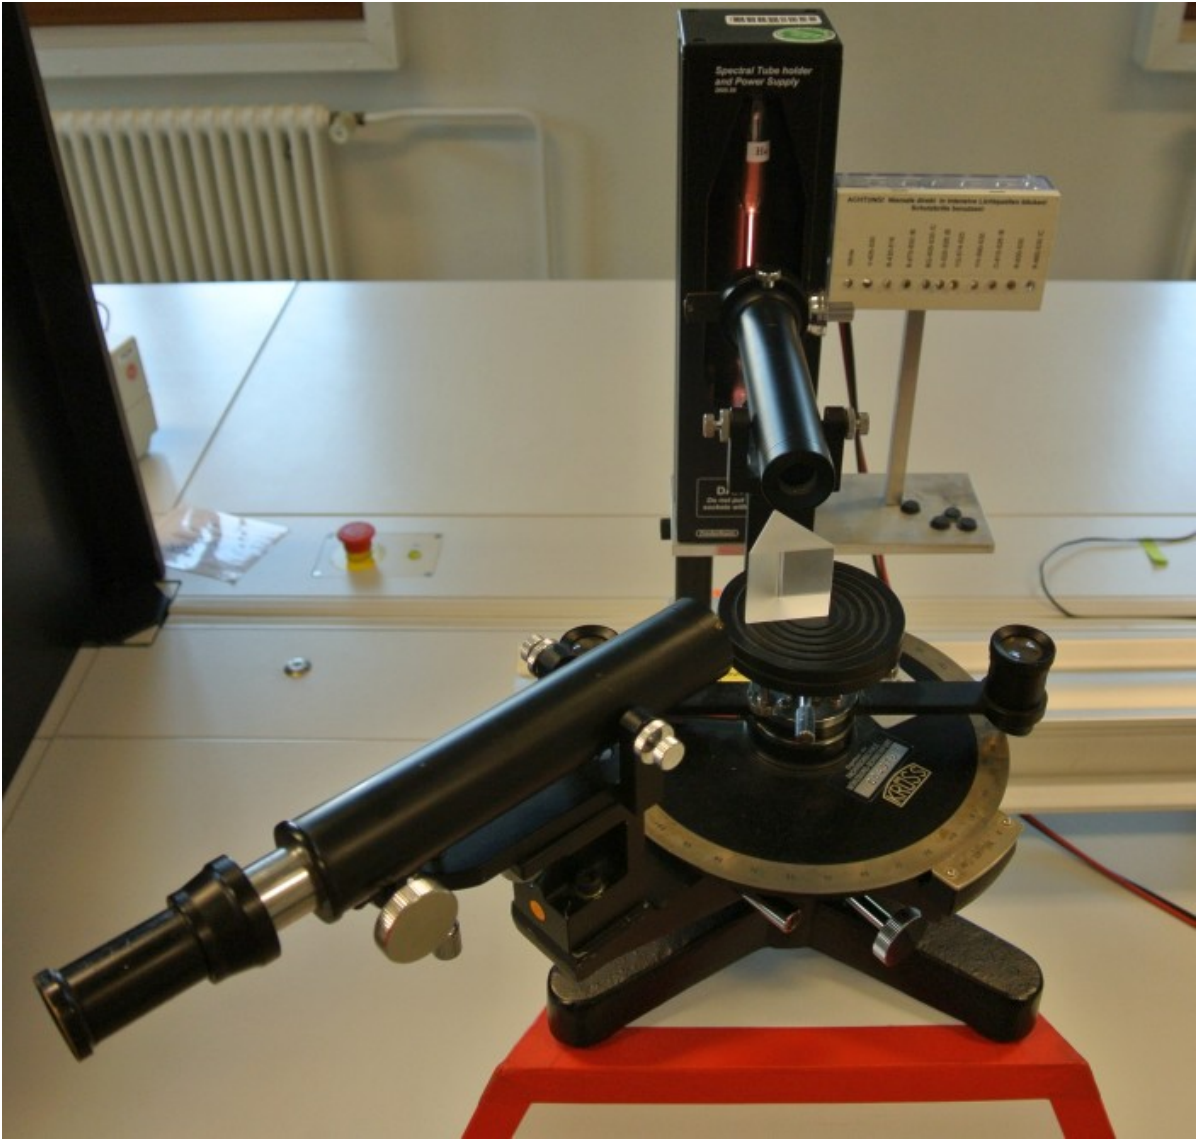
\includegraphics[width=8cm]{Abbildungen/Aufbau}
	\centering
	\caption{Veruchsaufbau Prismenspektrometer \cite{anl}}
	\centering
	\label{fig:Aufbau}
\end{figure}

\subsection{Durchführung}
Zuerst muss die Breite des Spaltes richtig eingestellt werden.
Anschließend wird die Teilkreisscheibe auf 0$^\circ$ 0' ausgerichtet und danach das Fernrohr auf 48$^\circ$ 0' positioniert.
Das Prisma wird zwischen Fernrohr und Spaltrohr platziert.
Abschließend wird die He-Lampe angeschaltet und das Fernrohr auf die Spektrallinie mit der größten Wellenlänge gestellt.
Aus dem Linienspektrum von Helium wird eine Referenzkurve ermittelt, mit der man jederzeit vom gemessenen Winkel auf die Wellenlänge schließen kann.

\newpage
\section{Auswertung Versuch}
\subsection{Helium-Lampe Referenzkurve}
Tabelle \ref{tab:Messwerte} zeigt die gemessenen Werte der He-Lampe.

\begin{table}[H]
	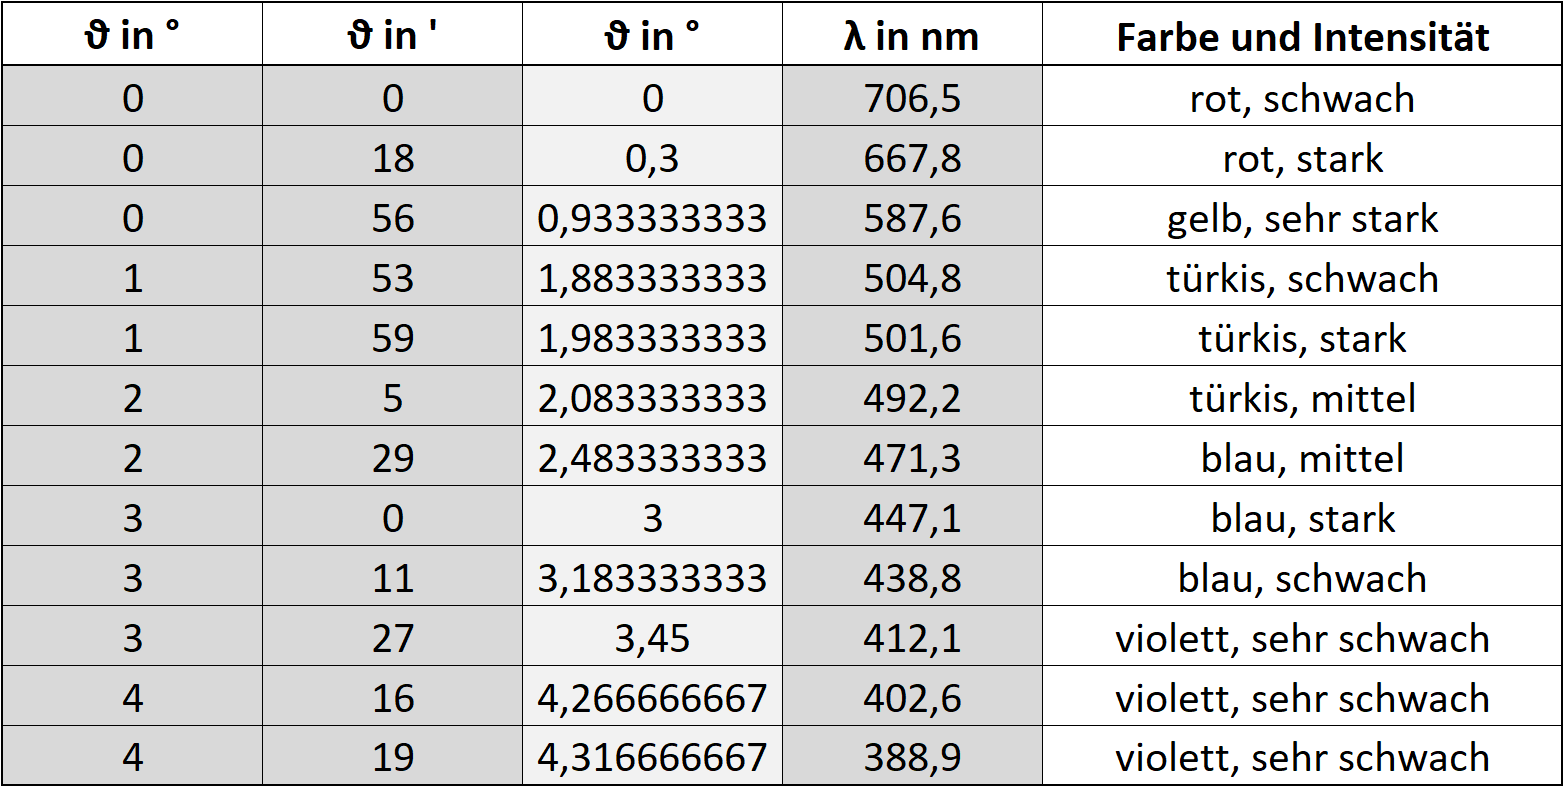
\includegraphics[width=14cm]{Abbildungen/Messwerte}
	\centering
	\caption{Messwerte an He-Lampe für Referenzkurve}
	\centering
	\label{tab:Messwerte}
\end{table}

Die Messunsicherheit für den Winkel $\vartheta$ beträgt:

\begin{align*}
	U_\vartheta = 5' = 0,083333^\circ
\end{align*}

Die daraus resultierende Referenzkurve ist in Abbildung \ref{fig:Diagramm} zu sehen.

\begin{figure}[H]
	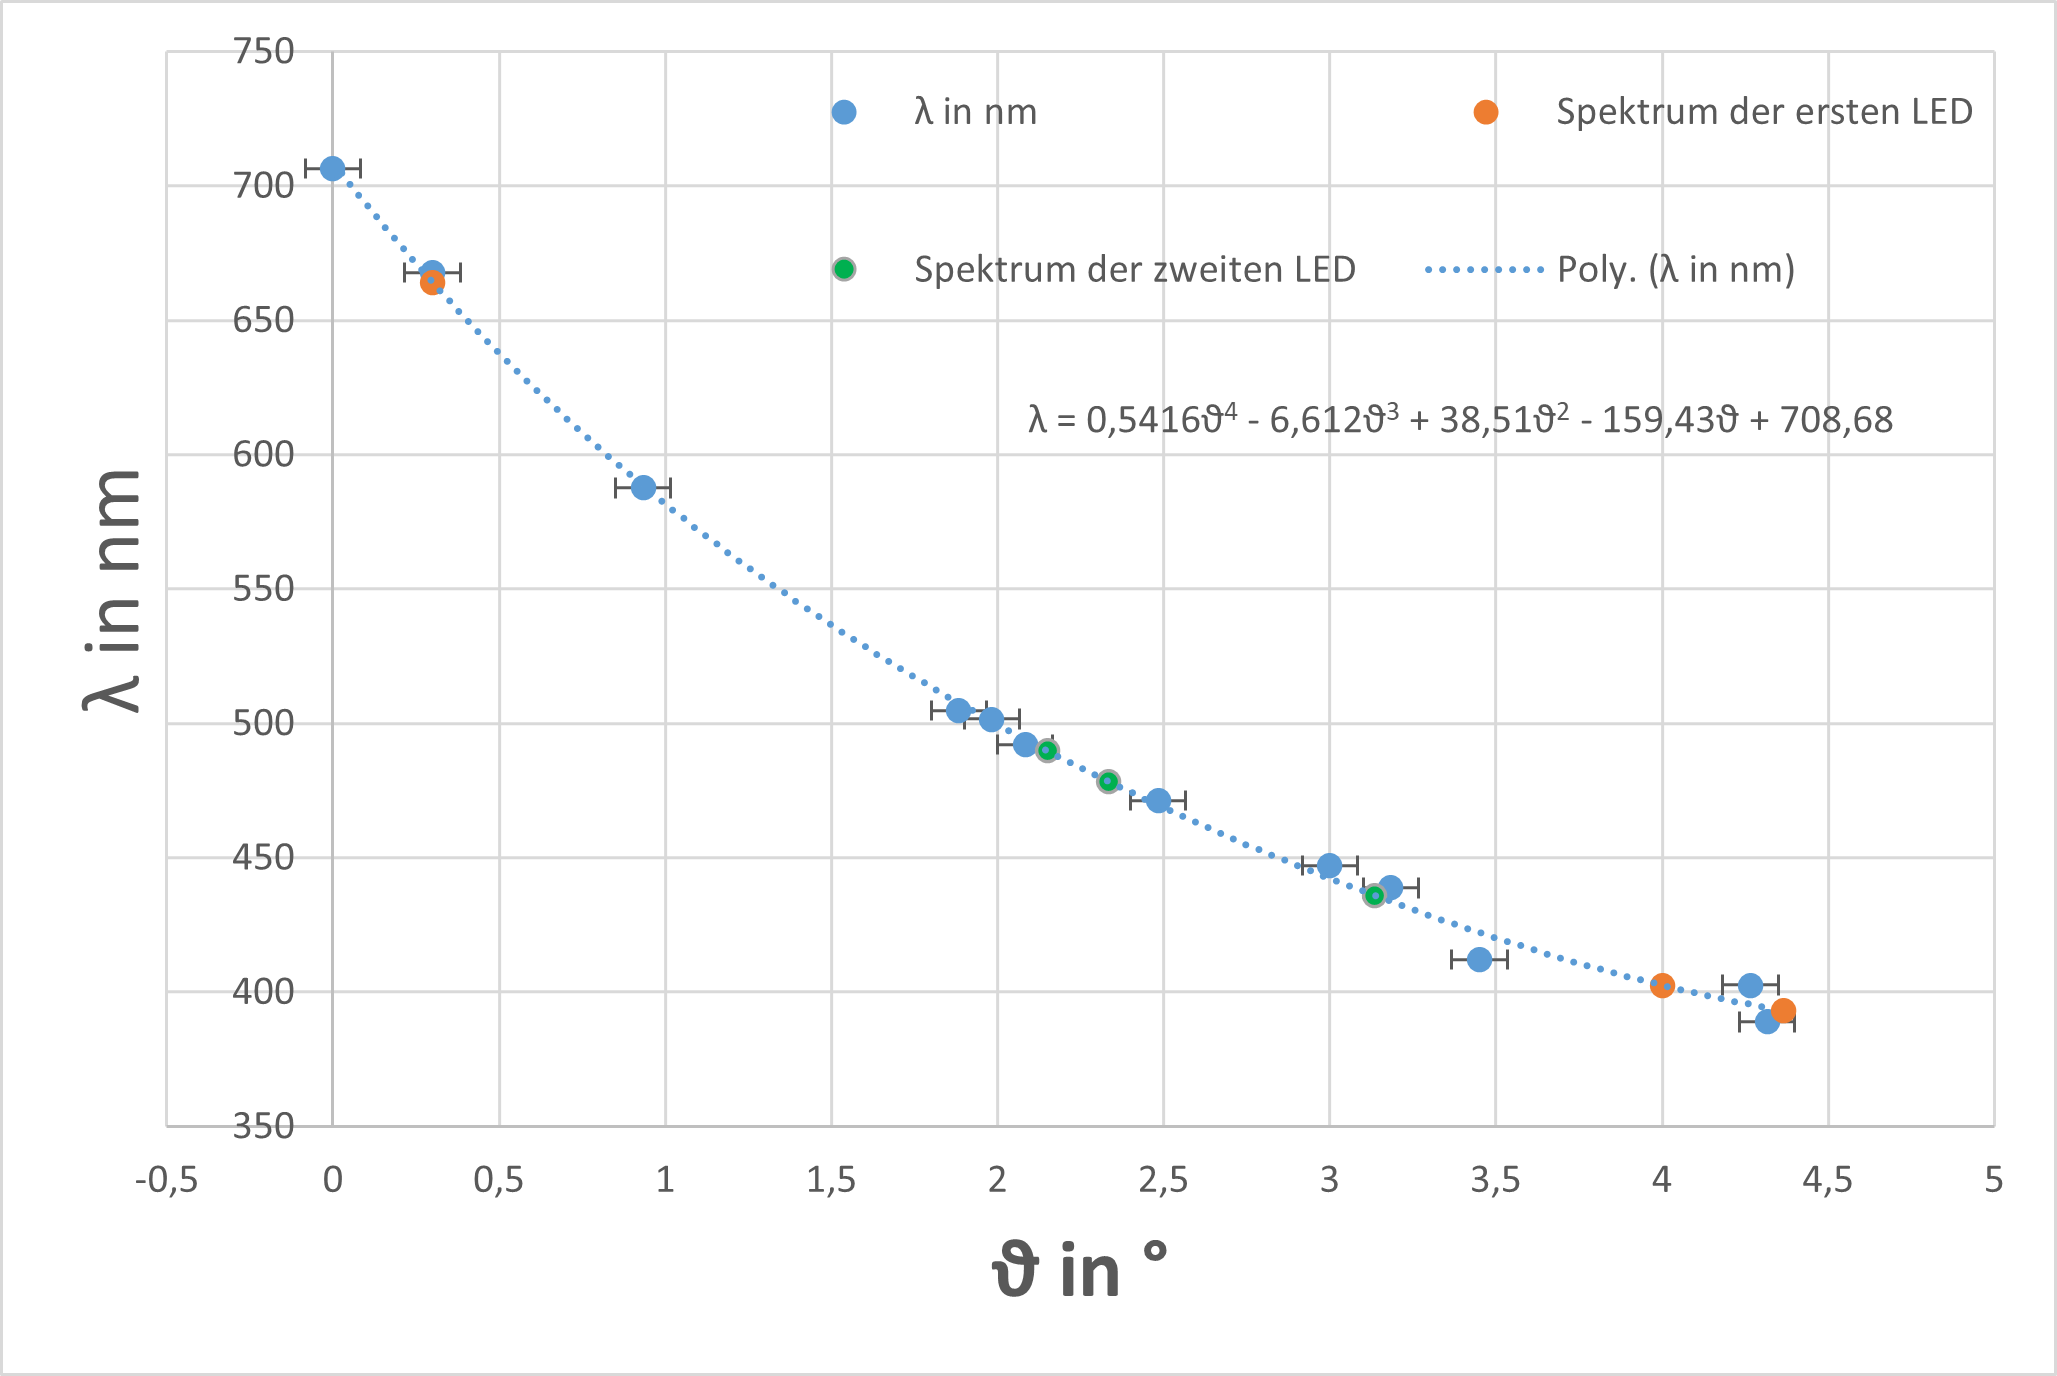
\includegraphics[width=14cm]{Abbildungen/Diagramm}
	\centering
	\caption{Referenzkurve Prismenspektrometer}
	\centering
	\label{fig:Diagramm}
\end{figure}
\newpage
Referenzkurve (polynomische Trendlinie 4. Grades):

\begin{align*}
	\lambda = 0,5416\vartheta^4 - 6,612\vartheta^3 + 38,51\vartheta^2 -159,43\vartheta + 708,68
\end{align*}

\subsection{Erste LED (Typ: V-405-530)}
Das Spektrum der ersten LED:

\begin{table}[H]
	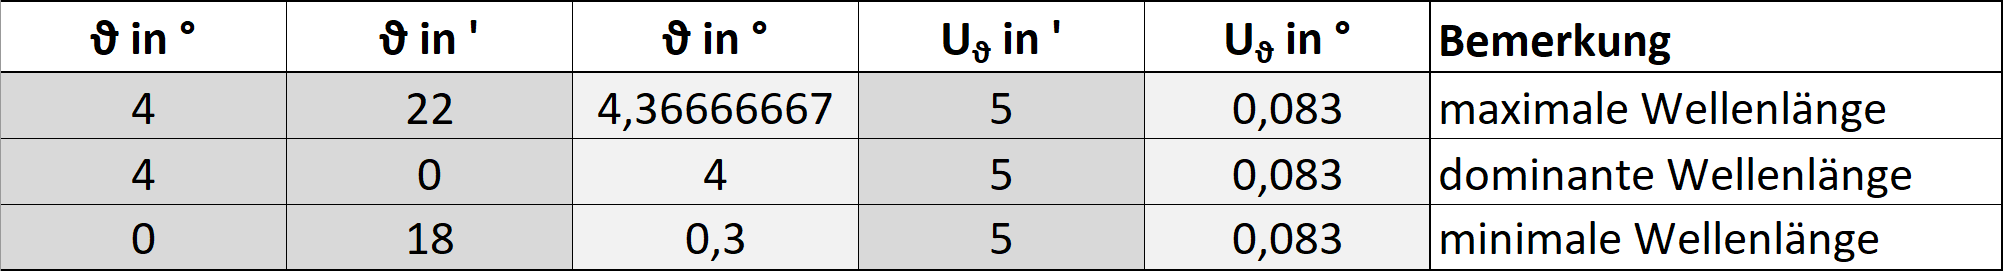
\includegraphics[width=14cm]{Abbildungen/MesswerteLED1}
	\centering
	\caption{Gemessene Werte für die erste LED}
	\centering
	\label{tab:MesswerteLED1}
\end{table}

Die in Tabelle \ref{tab:WellenlängeLED1} berechneten Messunsicherheiten wurden mithilfe der Fehlerfortpflanzung wiefolgt berechnet:

\begin{align*}
	\frac{\partial\lambda}{\partial\vartheta} = 4 \cdot 0,5416\vartheta^3 - 3 \cdot 6,612\vartheta^2 + 2 \cdot 38,51\vartheta -159,43
\end{align*}
\begin{align*}
	U_\lambda = \bigg | \frac{\partial\lambda}{\partial\vartheta} \bigg | \cdot U_\vartheta
\end{align*}

Mit Hilfe der Referenzkurve berechnete Wellenlängen:

\begin{table}[H]
	\includegraphics[width=10cm]{Abbildungen/WellenlängeLED1}
	\centering
	\caption{Berechnete Wellenlängen anhand der Referenzkurve}
	\centering
	\label{tab:WellenlängeLED1}
\end{table}

\subsection{Zweite LED (Typ: YG-574-520)}
Das Spektrum der zweiten LED:

\begin{table}[H]
	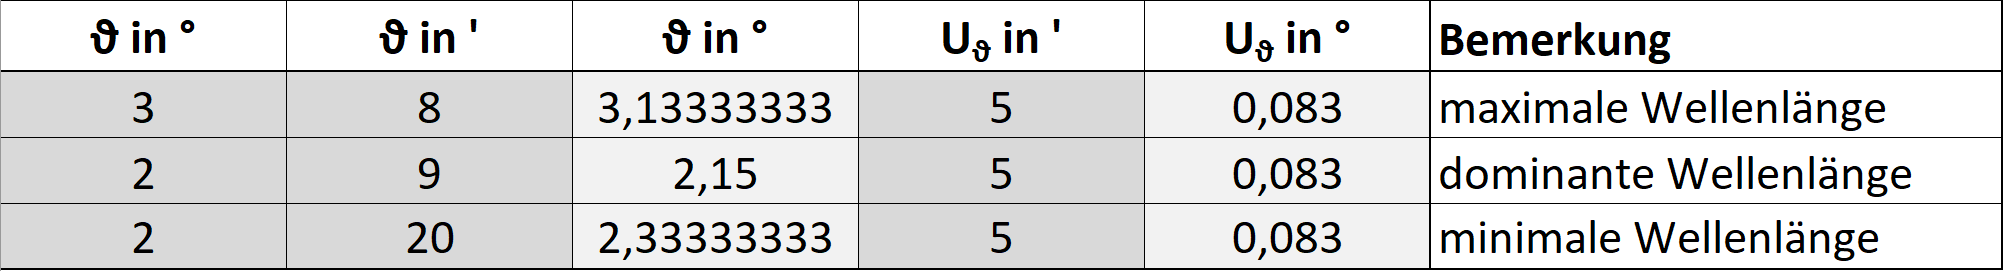
\includegraphics[width=14cm]{Abbildungen/MesswerteLED2}
	\centering
	\caption{Gemessene Werte für die zweite LED}
	\centering
	\label{tab:MesswerteLED2}
\end{table}
\newpage
Die in Tabelle \ref{tab:WellenlängeLED2} berechneten Messunsicherheiten wurden mithilfe der Fehlerfortpflanzung wiefolgt berechnet:

\begin{align*}
	\frac{\partial\lambda}{\partial\vartheta} = 4 \cdot 0,5416\vartheta^3 - 3 \cdot 6,612\vartheta^2 + 2 \cdot 38,51\vartheta -159,43
\end{align*}
\begin{align*}
	U_\lambda = \bigg | \frac{\partial\lambda}{\partial\vartheta} \bigg | \cdot U_\vartheta
\end{align*}

Mit Hilfe der Referenzkurve berechnete Wellenlängen:

\begin{table}[H]
	\includegraphics[width=10cm]{Abbildungen/WellenlängeLED2}
	\centering
	\caption{Berechnete Wellenlängen anhand der Referenzkurve}
	\centering
	\label{tab:WellenlängeLED2}
\end{table}


\newpage
\section{Wertung/Fazit}
Beim Versuch Prismenspektrometer waren sowohl bei der ersten als auch bei der zweiten LED Tendenzen zum Datenblatt zu erkennen.
Wenn man sich jetzt die dominanten Wellenlängen der gemessenen und im Datenblatt beschriebenen Werte anschaut, kommt man zu dem Fazit, dass es bei der ersten LED laut Statistik eine Überschneidung zwischen Herstel lerspezifikation (von dominant wavelength $U_{typ_{LED1}} = 405\;nm$) und der Messung (von $U_{LED1_{dominant}} = 402,6\pm2,5\;nm$) gab.
Daraus kann man folgern, dass die LED den Herstellerspezifikationen aus dem Datenblatt entspricht, da die Messung nicht das Gegenteil beweist.
\\
Bei der zweiten LED kommt es bei der Messung mit den Messunsicherheiten (von $U_{LED2_{dominant}} = 471,5\pm 4,7\;nm$) zu keiner Übereinstimmung mit dem Datenblatt (von dominant wavelength $U_{typ_{LED2}} = 574\;nm$).
Es kann sein, dass die LED außerhalb ihrer Spezifikationsgrenzen liegt, oder ungenau gemessen wurde.

\newpage
\bibliography{literatur}

\label{LastPage}

\end{document}
%%% Local Variables:
%%% mode: latex
%%% TeX-master: t
%%% End:
